\documentclass[border=10pt,tikz]{standalone}
\usepackage{amsmath}
\usetikzlibrary{calc}
\usetikzlibrary{decorations.pathmorphing} % for snakes
\usetikzlibrary {shapes.geometric} % for star
\usetikzlibrary{bending} % for arrow head angle
\usetikzlibrary{angles,quotes} % for pic (angle labels)
\usetikzlibrary{arrows.meta} % for arrow size

\usetikzlibrary {arrows}
\usetikzlibrary{shapes.geometric}
\begin{document}
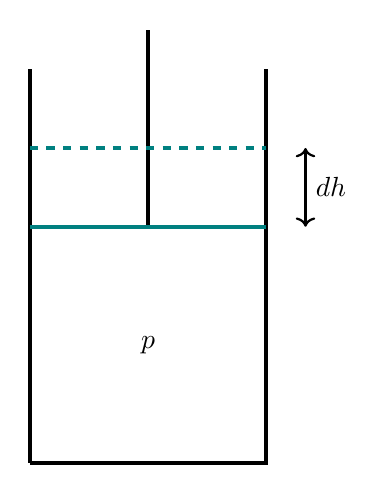
\begin{tikzpicture}[rotate=0]
    \coordinate (O) at (0,0);
    \coordinate (A) at (4,0);
    \coordinate (B) at (0,-4);
    \coordinate (P1) at (1,0);
    \coordinate (R2) at (4,-3.5);
    \draw[very thick] (0,0) -- (0, 5);
    \draw[ultra thick] (1.5,3) -- (1.5, 5.5);
    \draw[very thick] (0,0) -- (3, 0) -- (3, 5);
    \node[] at(1.5, 1.5) {$p$};
    \draw[ultra thick, teal] (0,3) -- (3, 3);
    \draw[very thick, dashed, teal] (0,4) -- (3, 4);
    \draw[<->, thick] (3.5, 3) -- node[right] {$dh$} (3.5, 4);
  \end{tikzpicture}
\end{document}